% Template for PLoS
% Version 3.5 March 2018
%
% % % % % % % % % % % % % % % % % % % % % %
%
% -- IMPORTANT NOTE
%
% This template contains comments intended
% to minimize problems and delays during our production
% process. Please follow the template instructions
% whenever possible.
%
% % % % % % % % % % % % % % % % % % % % % % %
%
% Once your paper is accepted for publication,
% PLEASE REMOVE ALL TRACKED CHANGES in this file
% and leave only the final text of your manuscript.
% PLOS recommends the use of latexdiff to track changes during review, as this will help to maintain a clean tex file.
% Visit https://www.ctan.org/pkg/latexdiff?lang=en for info or contact us at latex@plos.org.
%
%
% There are no restrictions on package use within the LaTeX files except that
% no packages listed in the template may be deleted.
%
% Please do not include colors or graphics in the text.
%
% The manuscript LaTeX source should be contained within a single file (do not use \input, \externaldocument, or similar commands).
%
% % % % % % % % % % % % % % % % % % % % % % %
%
% -- FIGURES AND TABLES
%
% Please include tables/figure captions directly after the paragraph where they are first cited in the text.
%
% DO NOT INCLUDE GRAPHICS IN YOUR MANUSCRIPT
% - Figures should be uploaded separately from your manuscript file.
% - Figures generated using LaTeX should be extracted and removed from the PDF before submission.
% - Figures containing multiple panels/subfigures must be combined into one image file before submission.
% For figure citations, please use "Fig" instead of "Figure".
% See http://journals.plos.org/plosone/s/figures for PLOS figure guidelines.
%
% Tables should be cell-based and may not contain:
% - spacing/line breaks within cells to alter layout or alignment
% - do not nest tabular environments (no tabular environments within tabular environments)
% - no graphics or colored text (cell background color/shading OK)
% See http://journals.plos.org/plosone/s/tables for table guidelines.
%
% For tables that exceed the width of the text column, use the adjustwidth environment as illustrated in the example table in text below.
%
% % % % % % % % % % % % % % % % % % % % % % % %
%
% -- EQUATIONS, MATH SYMBOLS, SUBSCRIPTS, AND SUPERSCRIPTS
%
% IMPORTANT
% Below are a few tips to help format your equations and other special characters according to our specifications. For more tips to help reduce the possibility of formatting errors during conversion, please see our LaTeX guidelines at http://journals.plos.org/plosone/s/latex
%
% For inline equations, please be sure to include all portions of an equation in the math environment.
%
% Do not include text that is not math in the math environment.
%
% Please add line breaks to long display equations when possible in order to fit size of the column.
%
% For inline equations, please do not include punctuation (commas, etc) within the math environment unless this is part of the equation.
%
% When adding superscript or subscripts outside of brackets/braces, please group using {}.
%
% Do not use \cal for caligraphic font.  Instead, use \mathcal{}
%
% % % % % % % % % % % % % % % % % % % % % % % %
%
% Please contact latex@plos.org with any questions.
%
% % % % % % % % % % % % % % % % % % % % % % % %

\documentclass[10pt,letterpaper]{article}
\usepackage[top=0.85in,left=2.75in,footskip=0.75in]{geometry}

% amsmath and amssymb packages, useful for mathematical formulas and symbols
\usepackage{amsmath,amssymb}

% Use adjustwidth environment to exceed column width (see example table in text)
\usepackage{changepage}

% Use Unicode characters when possible
\usepackage[utf8x]{inputenc}

% textcomp package and marvosym package for additional characters
\usepackage{textcomp,marvosym}

% cite package, to clean up citations in the main text. Do not remove.
% \usepackage{cite}

% Use nameref to cite supporting information files (see Supporting Information section for more info)
\usepackage{nameref,hyperref}

% line numbers
\usepackage[right]{lineno}

% ligatures disabled
\usepackage{microtype}
\DisableLigatures[f]{encoding = *, family = * }

% color can be used to apply background shading to table cells only
\usepackage[table]{xcolor}

% array package and thick rules for tables
\usepackage{array}

% create "+" rule type for thick vertical lines
\newcolumntype{+}{!{\vrule width 2pt}}

% create \thickcline for thick horizontal lines of variable length
\newlength\savedwidth
\newcommand\thickcline[1]{%
  \noalign{\global\savedwidth\arrayrulewidth\global\arrayrulewidth 2pt}%
  \cline{#1}%
  \noalign{\vskip\arrayrulewidth}%
  \noalign{\global\arrayrulewidth\savedwidth}%
}

% \thickhline command for thick horizontal lines that span the table
\newcommand\thickhline{\noalign{\global\savedwidth\arrayrulewidth\global\arrayrulewidth 2pt}%
\hline
\noalign{\global\arrayrulewidth\savedwidth}}


% Remove comment for double spacing
%\usepackage{setspace}
%\doublespacing

% Text layout
\raggedright
\setlength{\parindent}{0.5cm}
\textwidth 5.25in
\textheight 8.75in

% Bold the 'Figure #' in the caption and separate it from the title/caption with a period
% Captions will be left justified
\usepackage[aboveskip=1pt,labelfont=bf,labelsep=period,justification=raggedright,singlelinecheck=off]{caption}
\renewcommand{\figurename}{Fig}

% Use the PLoS provided BiBTeX style
% \bibliographystyle{plos2015}

% Remove brackets from numbering in List of References
\makeatletter
\renewcommand{\@biblabel}[1]{\quad#1.}
\makeatother



% Header and Footer with logo
\usepackage{lastpage,fancyhdr,graphicx}
\usepackage{epstopdf}
%\pagestyle{myheadings}
\pagestyle{fancy}
\fancyhf{}
%\setlength{\headheight}{27.023pt}
%\lhead{
\includegraphics[width=2.0in]{PLOS-submission.eps}}
\rfoot{\thepage/\pageref{LastPage}}
\renewcommand{\headrulewidth}{0pt}
\renewcommand{\footrule}{\hrule height 2pt \vspace{2mm}}
\fancyheadoffset[L]{2.25in}
\fancyfootoffset[L]{2.25in}
\lfoot{\today}

%% Include all macros below

\newcommand{\lorem}{{\bf LOREM}}
\newcommand{\ipsum}{{\bf IPSUM}}


% Pandoc citation processing
\newlength{\csllabelwidth}
\setlength{\csllabelwidth}{3em}
\newlength{\cslhangindent}
\setlength{\cslhangindent}{1.5em}
% for Pandoc 2.8 to 2.10.1
\newenvironment{cslreferences}%
  {}%
  {\par}
% For Pandoc 2.11+
\newenvironment{CSLReferences}[2] % #1 hanging-ident, #2 entry spacing
 {% don't indent paragraphs
  \setlength{\parindent}{0pt}
  % turn on hanging indent if param 1 is 1
  \ifodd #1 \everypar{\setlength{\hangindent}{\cslhangindent}}\ignorespaces\fi
  % set entry spacing
  \ifnum #2 > 0
  \setlength{\parskip}{#2\baselineskip}
  \fi
 }%
 {}
\usepackage{calc} % for calculating minipage widths
\newcommand{\CSLBlock}[1]{#1\hfill\break}
\newcommand{\CSLLeftMargin}[1]{\parbox[t]{\csllabelwidth}{#1}}
\newcommand{\CSLRightInline}[1]{\parbox[t]{\linewidth - \csllabelwidth}{#1}\break}
\newcommand{\CSLIndent}[1]{\hspace{\cslhangindent}#1}




\usepackage{forarray}
\usepackage{xstring}
\newcommand{\getIndex}[2]{
  \ForEach{,}{\IfEq{#1}{\thislevelitem}{\number\thislevelcount\ExitForEach}{}}{#2}
}

\setcounter{secnumdepth}{0}

\newcommand{\getAff}[1]{
  \getIndex{#1}{Universitat de Barcelona (UB),Vall d'Hebron Research
Institute (VHIR)}
}

\providecommand{\tightlist}{%
  \setlength{\itemsep}{0pt}\setlength{\parskip}{0pt}}

\begin{document}
\vspace*{0.2in}

% Title must be 250 characters or less.
\begin{flushleft}
{\Large
\textbf\newline{\emph{A heuristic algorithm to select genes potentially
regulated by
methylation}} % Please use "sentence case" for title and headings (capitalize only the first word in a title (or heading), the first word in a subtitle (or subheading), and any proper nouns).
}
\newline
% Insert author names, affiliations and corresponding author email (do not include titles, positions, or degrees).
\\
Alex Sanchez-Pla\textsuperscript{\getAff{Universitat de Barcelona
(UB)}, \getAff{Vall d'Hebron Research Institute
(VHIR)}}\textsuperscript{*},
Berta Miro\textsuperscript{\getAff{Vall d'Hebron Research Institute
(VHIR)}}\\
\bigskip
\textbf{\getAff{Universitat de Barcelona (UB)}}Departament of Genetics
Microbiology and Statistics, Avda Diagonal 645, Barcelona, 08028\\
\textbf{\getAff{Vall d'Hebron Research Institute (VHIR)}}Statistics and
Bioinformatics Unit (UEB), Passeig de la Vall d'Hebron 119-129,
Barcelona, 08035\\
\bigskip
* Corresponding author: asanchez@ub.edu\\
\end{flushleft}
% Please keep the abstract below 300 words
\section*{Abstract}
Methylation is a key process in cancer that usually acts by inhibiting
gene expression. However, when methylation is low, any value range can
be found for gene expression in a given gene. This would suggest that,
to select genes regulated by methylation, one may look for patterns in
the relationship between gene expression and methylation that either
show a negative correlation or a more pronounced ``L-shape.'' To that
end, we have developed a heuristic algorithm that mimics the process of
visually selecting an ``L-shape.'' In this algorithm, when methylation
is low, selected genes may exhibit a wide range of expression values
(from low to high), but only low gene expression is selected for high
methylation. The method has been implemented in an R package,
\texttt{Lheuristic} and a Shiny application, both available from GitHub
(http://github.com/alexsanchezpla). For two given matrices - one for
expression and one for methylation with matched values for row and
column names - the program offers the possibility to select genes based
on either negative correlation, the heuristic algorithm or both methods
at once. Once genes have been selected, results can be interactively
reviewed, plotted and also downloaded. The method shows good performance
when compared against the naïve correlation, especially due to its
flexibility.

% Please keep the Author Summary between 150 and 200 words
% Use first person. PLOS ONE authors please skip this step.
% Author Summary not valid for PLOS ONE submissions.

\linenumbers

% Use "Eq" instead of "Equation" for equation citations.
\hypertarget{introduction-and-background}{%
\section{Introduction and
Background}\label{introduction-and-background}}

\hypertarget{introduction-to-methylation}{%
\subsection{Introduction to
methylation}\label{introduction-to-methylation}}

Epigenetic marks modulate gene expression without affecting the DNA
nucleotide sequence. These potentially heritable changes are, for
example, DNA methylation or histone acetylation ({[}1{]}). DNA
methylation is the most studied epigenetic process in humans. The
process is based on the addition of a methyl group, mostly in CpG
dinucleotides. The CpG dinucleotides tend to group in areas of less than
500kb and with higher than 55\% C and G content, these regions are named
islands; further from the island the region is called shore; and further
from the shore it is called shelf. More than 60\% of promoter regions
are associated with CpG islands ({[}2{]}) and the methylation of these
is linked to gene silencing and gene expression inhibition. DNA
methylation has been linked to the regulation of numerous cellular
processes, including embryonic development, or X-chromosome inactivation
and preservation of chromosome stability among others. DNA methylation
has also been observed in autoimmune diseases, metabolic disorders,
neurological disorders, and other processes that despite being natural
they are debilitating, like ageing for example; and it can also be
correlated with drug or treatment response ({[}3{]}; {[}4{]}; {[}5{]};
{[}6{]}). Most research on this area has been, however, focused on tumor
repressor genes, which are often silenced in cancer cells due to
hypermethylation. This is an important mechanism of gene silencing
during tumor progression ({[}7{]}). On the contrary, a general level of
hypomethylation has been observed in human tumors ({[}8{]}); therefore,
hypomethylation is a useful mechanism to distinguish genes of some human
cancers from their normal counterparts.\\
In the human genome, about 80\% of cytosines in the 56 million CpG sites
are methylated to 5-methylcytosines. The methylation pattern of DNA is
highly variable among cells types and developmental stages and
influenced by disease processes and genetic factors. The relationship
between gene expression and methylation has been associated with cancer
and extensively studied, therefore it has produced fruitful results
({[}9{]}).

\hypertarget{analysis-of-genes-regulatated-by-methylation}{%
\subsection{Analysis of genes regulatated by
methylation}\label{analysis-of-genes-regulatated-by-methylation}}

With the abundance of emerging evidence indicating the important role of
DNA methylation in common diseases, researchers have attempted to use
DNA methylation as a biomarker to identify epigenetic changes that are
associated with disease status. While the genetic events that drive the
tumorigenic process are relatively well characterized for colorectal
cancer, the epigenetic events and their impact on the transcriptional
reprogramming observed in colorectal tumors have not been extensively
characterized. Although recent genome-wide studies have analyzed the
genomic distribution of hypermethylated CpGs in a small number of
colorectal tumors ({[}10{]}; {[}11{]}; {[}12{]}), a detailed analysis of
the subset of these events that are important for gene expression
regulation is currently lacking. Just as gene expression microarrays
accelerated and revolutionized the study of transcriptional regulation,
rapidly improving technologies are increasingly enabling researchers to
assess locus-specific DNA methylation on a genome-wide scale. Recently,
various high-throughput approaches based on bisulfite conversion, that
combined with next generation sequencing, have been developed and
applied for the genome wide analysis of DNA methylation. These methods
provide single base pair resolution, quantitative DNA methylation data
with genome wide coverage. There are various experimental types of
methylation assays, but overall, methylation levels can be represented
in one of three types: discrete, continuous or categorical. Therefore,
methylation can be quantified by directly using read count information,
ratio data (which may lose biological variability) or both. Once the DNA
samples are processed, an important issue to be considered is the
influence of the statistical analysis on the accuracy of the genomic
methylation level estimation from bisulfite sequencing data. The
accuracy of the statistical approach to methylation quantification
increases with the sequencing depth of the particular cytosine residue
({[}13{]}). However, there are regression and neighboring analysis
techniques that can counteract the lack of sequence depth in a
particular CpG ({[}14{]}).

\hypertarget{existing-methods-and-analyses}{%
\subsubsection{Existing methods and
analyses}\label{existing-methods-and-analyses}}

The association between gene expression and DNA methylation in the CpG
islands in particular has been long studied. As a result, mostly
negative correlations have been found to relate to cancer driven
mechanisms ({[}15{]}). Nevertheless, this inverse relationship between
DNA methylation, of the first intron in particular, and gene expression
is a broad mechanism to down-regulate gene expression and it is found in
numerous processes, organisms and tissues ({[}16{]}). There have been
various studies analysing this correlation using diverse approaches. For
example, Massie et al.~(2017) looked at the relationship between gene
expression and DNA methylation at the probe level rather than at the
gene level. They narrowed a list of genes regulated by methylation that
were identified in more than 3 out of 17 studies ({[}17{]}). Another
study analysed the TCGA database to identify patterns in DNA CpG
methylation and gene expression and tumor status. They found that the
association involved a reduced number of genes linked to cancer than
originally anticipated (around the hundreds) and that not all
correlations were negative ({[}18{]}). Another recent paper reported two
different models for analysis of DNA methylation and regulation of gene
expression, one for negatively correlated genes and one for positively
correlated genes ({[}19{]}). They used expression (GSE106582) and
methylation datasets (GSE101764) containing 194 samples, 77 tumors and
117 of the mucose. By random forest analysis they were able to classify
genes into cancer related and not related. Still methodologies to find
tune classification into cancer/disease related and not cancer/disease
related are still needed. A previously developed method was the
selection of genes with an L-shape association between the expression
and the methylation datasets ({[}20{]}). In this research, they focused
on the CMI (Conditional Mutual Information) metric and on another method
based on spline regression. They observed that the first method would
detect L-shaped genes more accurately in big datasets. On the other
hand, the splines clustering was not size dependent, but it would yield
a smaller number of samples. Other research exists that aimed to
identify genes regulated by methylation according to the
expression/methylation patterns; however, they only use a particular
methodology like the CMI ({[}21{]}) with positive results. A paper
focused on the identification of genes regulated by methylation through
unsupervised clustering techniques to identify CRC subtypes was able to
confirm existing subtypes ({[}22{]}).There has been other work that
focused on the development of platforms for the identification of genes
regulated by methylation. One of these packages is MEXPRESS ({[}23{]}).
This package has a web interface that allows the user to visualize
expression and methylation data from genes in the TCGA data. The
visualization collocates for each selected gene, CpG islands, with
transcripts expression together with other clinical values such as
gender and age. The tool also generates p-values in relation to the
variables specified. Another one of these packages is MethylMix, based
in R ({[}24{]}). The algorithm is based on a beta mixture model that
identifies methylation states and compares them with what they call
normal conditions to find hypo- and hyper-methylated genes. They
developed a new statistic coefficient, the Differential Methylation
value or DM-value which is defined as the difference of a methylation
state with the normal methylation state. Then, they correlate that
coefficient with gene expression data to characterize the association
between the methylation level and gene expression. ELMER
(https://bioconductor.org/packages/release/bioc/html/ELMER.html,
{[}25{]}) is another R package that performs an integrative analysis of
methylation and gene expression using the difference of methylation
between control and deseased samples to select differentially methylated
probes. These selected probes are then aligned to each downstream gene
targets; and finally, the predicted enhancers are integrated to
expression data and a selection is generated by negative correlation
analysis (either supervised or unsupervised). There is also a web based
tool that analyses methylated genes based on TCGA data, called MethHC
(http://methhc.mbc.nctu.edu.tw/php/search.php?opt=gene, {[}26{]}). This
database has an analysis tool that provides gene-specific analysis for
various diseases, and the information is displayed as a comparison
between diseased and normal (non-diseased) conditions; list of highest
and lowest methylated (hyper and hypo) genes; as well as correlations
between expression and methylation. In this, methylation is considered
as a binary value (0,1). There have been other methodologies used to
identify methylated genes associated with cancer is through text mining
analysis, as in the PubMeth database (www.pubmeth.org, {[}27{]}). In
this, they identified 5000 genes from 1000 publications. However,
high-throughput methodologies that offer an impartial approach to the
identification of genes regulated by methylation still need further
development and fine-tuning. Here we present such a methodology to
select, out of a gene expression and DNA methylation subsets, those
genes that not only present a negative correlation, but also have a
particular ``L-shape'' and are therefore potentially regulated by
methylation. The L-shaped heuristic method developed to identify genes
regulated by methylation was tested and tuned for experimental
expression and methylation paired datasets previously normalized.

\hypertarget{materials-and-methods}{%
\section{Materials and Methods}\label{materials-and-methods}}

As previously described, there are various approaches to selecting genes
based on the relationship between methylation levels and gene
expression;however, none of them are completely satisfactory.

In this section we present the method we have developed to select genes
in which the pattern of the relationship is ``L-shaped.'' In fact,
taking biological processes into account, this is a very common and very
reasonably expected pattern when genes are regulated by methylation.
Furthermore, as we will see later, it is not only important but can be
partially missed by ``naïve'' methods such as negative correlation,
which increases the interest of our proposed methodology.

\hypertarget{rationale-of-the-approach}{%
\subsection{Rationale of the approach}\label{rationale-of-the-approach}}

After trying different approaches to detect L-shapes, one often comes
back to an intuïtive idea: If we are looking for genes whose expression
can take any value when methylation is low, and tends to decrease as
methylation increases one should observe that points in the
methylation-expression scatterplot tend to be scattered near the
vertical and horizontal positive axes showing an L-shape. If this does
not happen genes can be found anywhere in the scatterplot and we can
call it a non-L-shape. That is:

\begin{itemize}
\tightlist
\item
  The more the points cluster near the vertical and horizontal axes, the
  more L-shaped can be considered the scatterplot.
\item
  The more the points move away from the axes, the least L-shaped the
  scatterplot is.
\end{itemize}

This representation of differing scatterplot patterns can be observed in
two real but non-identified genes from a colorectal cancer study (Fig.
1).

\hypertarget{an-algorithm-to-select-l-shape-scatterplots}{%
\subsection{An algorithm to select L-shape
scatterplots}\label{an-algorithm-to-select-l-shape-scatterplots}}

Assuming that genes potentially regulated by methylation can be selected
from between L-shaped expression--methylation scatterplots, finding a
way to separate L-shape from non-L shape ones is a reasonable first
step. It could be argued that this could be done manually, but given the
high number of -possibly highly variable- figures to be searched, an
algorithm to automate this process is a much better option.

The algorithm can be developed starting from the intuitive distinction
between L and non-L discussed above and making it more explicit as
follows:

\begin{enumerate}
\item Given a scatterplot methylation-expression $X$, overlay a $k\times m$ grid on it so that each point is assigned to one and only one of the grid's cell. Usually $k=m=3$ so this will be the values used in the following.
\item Classify the scatterplot as \textbf{``L'' or ``non-L''} based on a small set of conditions:
\begin{enumerate}
  \item There must be a \emph{minimum} number of points in the upper-left (cell (1,1)) and lower right (cell (3,3)) corners of the grid.
  \item There must be a \emph{maximum} number of points in the upper right (cell (1,3)) because points there mean hypermethylation and hyperexpression which is the opposite of what we are looking for.
  \item We will usually \emph{not require to have a minimum of points in cell (3,1)} unless we are really willing to have an L-shape (in our setting we will also be happy tho recover diagonals, which also reflect a negative correlation!).
\end{enumerate}
\item Score points on each subgrid in such a way that
\begin{enumerate}
    \item Points in permitted regions (left-outer margin, i.e. cells: (1,1), (2,2), (3,1), (3,2), (3,3)) score positively if the scatterplot has been classified as L or zero if it has been classified as non-L.
    \item Points in non-desired regions (outer band. i.e. cells (1,2), (1,3), (2,3)) score negatively in all cases.
    \item Some regions may be declared neutral and not-score, such as cell (2,2).
\end{enumerate}
\item Use cross-validation to tune scoring parameters (\textit{if a set of positive and negative L-shaped genes is available}). 
\end{enumerate}

The previous scheme can be summarized using the following equation.
\begin{equation}
S(X) = W_L \circ X \times \mathbf{1}_L(X) + W_{L^C} \circ X \times \mathbf{1}_{L^c}(X),
\end{equation} where

\begin{itemize}
\item ${X}$ is the matrix of \emph{counts}, i.e. the number of counts in each cell of the grid,
\item ${W_L}$ is the matrix of scores per cell and point \emph{if the scatterplot has been classified as $L$},
\item ${W_{L^c}}$ is the matrix of scores per cell and point \emph{if the scatterplot has been classified as non-$L$ ($L^c$)},
\end{itemize}

and \(\circ\) represents the hadamard product of the two matrices
\(W_{L/L^c}\) (i.e.~elementwise multiplication of the two matrices) and
\(\mathbf{1}_{L/L^c}()\) is the indicator function for \(L\) or \(L^c\).

The fact that the scatterplot is assigned to \(L\) or \(L^c\) can also
be described as the hadamard product of three matrices: \begin{equation}
\mathbf{1}_L(X) = \bigwedge_{i,j} X \circ C \circ \left( mMP \times \sum_{i,j}x_{ij}\right),
\end{equation} where

\begin{itemize}
\item ${X}$ is the matrix of \emph{counts}, i.e. the number of counts in each cell of the grid,
\item $C$ is the matrix of conditions to be verified \emph{if the scatterplot has to be classified as $L$},
\item $mMP$ is the matrix of minimum and Maximum Percentages of points to have in each cell \emph{if the scatterplot has to be classified as $L$},
\item $\circ$ represents the pointwise logical operation which allows that the product of the three cells becomes a logical operation and
\item $\bigwedge_{i,j}$ represents an logical ``AND'' operation of all cells, that is if all cells are TRUE the result is assigned to $L$ and if one fails it is assigned to $L^c$.
\end{itemize}

Fig. 2 shows a graphic representation of this grid approach.

\hypertarget{data-sources}{%
\subsection{Data sources}\label{data-sources}}

\hypertarget{tcga-coad-datasets}{%
\subsubsection{TCGA-COAD datasets}\label{tcga-coad-datasets}}

The TCGA-COAD are a group of datasets from the colon adenocarcinoma
project, which contains data from both the colon and the rectosigmoid
junction. It has 452 cases for expression datasets and 451 for
methylation. Data was downloaded from the TCGA database
(https://www.cancer.gov/about-nci/organization/ccg/research/structural-genomics/tcga).
The final dataset used for analysis with the heuristic classification
method after matching both cases and genes for expression and
methylation had 223 patient samples and 11788 genes in common.

\hypertarget{crc-experimental-reserach-datasets}{%
\subsubsection{CRC experimental reserach
datasets}\label{crc-experimental-reserach-datasets}}

An experimental dataset was used from the study (Diego Arango article),
which contained a total of 30 samples and 11359 genes.

\hypertarget{synthetic-dataset-generation-for-the-simulation-studies}{%
\subsubsection{Synthetic dataset generation for the simulation
studies}\label{synthetic-dataset-generation-for-the-simulation-studies}}

The R package \texttt{simstudy} was used to create 4 artificial datasets
by using the splines method
(https://cran.r-project.org/web/packages/simstudy/simstudy.pdf). The
package allows for designing data points on a pre-defined spline, in
which knots, limits and dispersion can be tuned. The splines were
generated based on a fixed X variable representing the methylation
values. The artificial datasets contained a total of 1000 genes, and the
data points were developed based on 2 parameters with 2 levels each. The
first parameter was the number of samples and the second the \% of genes
with an expression by methylation scatterplot or spline following an
L-shape (potentially regulated by methylation) that a sample would
contain. The number of samples or cases considered was of 50 and 1000,
and the \% of L-shaped genes in each dataset was 1\% and 10\%.
Additionally, the shape of the negative genes (potentially not regulated
by methylation) was also pre-defined and classified into 5 different
scatterplot patterns (Fig. 3). The percentage of genes in each category
equaled to 1/3 prior subtraction of the L-shaped genes. These artificial
genes were generated based on real gene patterns observed from previous
analyses with TCGA and experimental CRC data (Fig. 4).

\hypertarget{results}{%
\section{Results}\label{results}}

\hypertarget{presentation-of-method-parameters-input-and-output}{%
\subsection{Presentation of method parameters, input and
output}\label{presentation-of-method-parameters-input-and-output}}

\hypertarget{manin-functions-and-parameters}{%
\subsubsection{Manin functions and
parameters}\label{manin-functions-and-parameters}}

The scoreGenesMat is a wrapper function that generates and scores any
given scatterplot using a binary and a numeric schemes on a row-wise
basis Parameters required to run the analysis with the scoreGenesMat
function:

\begin{itemize}
\tightlist
\item
  \textbf{mets} Matrix of methylation values
\item
  \textbf{expres} Matrix of expression values
\item
  \textbf{aReqPercentsMat} Matrix of minimum maximum percentage of
  counts to have in a given cell
\item
  \textbf{aWeightMifL} A matrix of weights to score the previous counts
  if the scatterplot has been classified as L.
\item
  \textbf{aWeightMifNonL} A matrix of weights to score the previous
  counts if the scatterplot has been classified as non-L
\end{itemize}

PARAMETROS QUE HEREDA (O NO) DE CALCFREQS * \textbf{x1, x2}, Coordinates
of vertical points in the X axis. Because it is expected to contain
methylation values that vary between 0 and 1 the default values are 1/3
and 2/3. * \textbf{y1, y2}, Coordinates of vertical points in the Y
axis. Leaving them as NULL assigns them the percentiles of yVec defined
by \texttt{percY1} and \texttt{percY2}. * \textbf{percY1, percY2} Values
used to act as default for \texttt{y1}and \texttt{y2} when these are set
to \texttt{NULL} * \textbf{trace} Set to TRUE to print count matrices as
they are computed

standardWeightMifL \textless- matrix (c(2,-2,-100,1, 0,-2, 0, 0, 0),
nrow=3, byrow=TRUE) standardWeightMifNonL \textless- matrix
(c(0,-2,-100,0, 0,-2, 0, 0, 0), nrow=3, byrow=TRUE) standardPercentsMat
\textless- matrix (c(10, 20, 0, 5, 0, 20, 0, 5, 10), nrow=3, byrow=TRUE)

\hypertarget{input}{%
\subsubsection{Input}\label{input}}

Expression dataset Methylation dataset

Data preprocessing

\hypertarget{results-1}{%
\subsubsection{Results}\label{results-1}}

\begin{itemize}
\tightlist
\item
  \texttt{logicSc}: TRUE o FALSE segun si se cumplen los criterios
  definidos para el método Heuristic
\item
  \texttt{numericSc}; Puntuación obtenida por el metodo heurístico.
\end{itemize}

Genes considerados en forma de L Las tablas de resultados tan sólo
generan un valor binario para el método heurístico, por ejemplo
definiremos ``Regulado por metilación'': Si no se incumplen los
porcentajes fijados en ninguna celda (\texttt{logicSc=TRUE}).

\begin{itemize}
\tightlist
\item
  list of selected genes
\item
  graphs
\item
  intersection of lists (venn)
\end{itemize}

\hypertarget{performance-evaluation-in-the-heuristic-method}{%
\subsection{Performance evaluation in the heuristic
method}\label{performance-evaluation-in-the-heuristic-method}}

There is a limitation to evaluate the type I and type II errors of the
results generated due to the lack of a set of ``TRUE Positives'' -genes
in the datasets analyzed proven to have L-shape- or ``TRUE negative''
genes known not to have L-shape- due to the difficulty to obtain these
parameters from experimental samples. Therefore, an approach to perform
a selection between the TRUE and FALSE genes is by visually inspecting
the genes and selecting two sets that can be described as ``clearly L''
and ``clearly non-L.'' Even though this strategy fairly accurate, it is
a difficult concept to execute programatically, with the added
subjectivity to the selection. For example, there are samples with
intermediate scatterplot shapes that are not ``clear.'' To attempt to
override that, two strategies were followed. On one hand, synthetic
datasets were created based on results obtained from real datasets (TCGA
and experimental dataset). As the synthetic datasets were designed based
on experimental TRUE and FALSE patterns, they were used as reference to
assess the method's performance. On the other hand, a common dataset
from TCGA was used to compare our model to 2 other software solutions
that also select hypomethylated genes from the integration of gene
expression and methylation.

The first approach was to assess the heuristic model's performance with
the 4 synthetic datasets with the predefined parameters described in the
section above.The datasets used had respectively 50 samples and 1\% of
``known'' L-shaped genes; 50 and 10\%; 1000 and 1\%; and 1000 and 10\%,
all with 1000 genes in total. Since the genes that had an L-shaped were
know, as they had been synthetically designed, the results were used to
adjust some model parameters. The parameters tested were the following:

\begin{itemize}
\tightlist
\item
  x1, x2: grid partition into 3x3 and 4x4 on the X axis
\item
  percY1, percY2: grid partition into 3x3 and 4x4 on the Y axis
\item
  aWeightMifL: 3 parameter options were considered at each point
\item
  aReqPercentsMat: 2 parameter options were considered at each point
\end{itemize}

Regarding \textbf{x1, x2, percY1, percY2}, the grid division in to 1/3
generating a 3x3 matrix provided optimal results. Adjusting the selected
parameters of the \textbf{aWeightMifL} matrix did not change the
results. Four parameters of the \textbf{aReqPercentsMat} did change both
error type I and type II. These parameters were x3, x4, x8 and x9.

Using the optimal parameter combinations, the identification of L-shaped
genes was of 10 for the 1\% and 50 samples dataset, 100 L-shaped genes
for the 10\% and 50 samples, 8 gene for the the 1\% and 1000 samples,
and 88 L-shaped genes for the 1\% and 1000 samples. The false positives
were 45, 0, 1, and 0, respectively. The false negatives were 90, 42, 2,
and 12, respectively.

All parameter combinations and respective count matrices for L and NoL
genes can be found in the Supplementary table xxx.

\hypertarget{tuning-of-parameters-to-evaluate-and-improve-method-performance}{%
\subsubsection{Tuning of parameters to evaluate and improve method
performance}\label{tuning-of-parameters-to-evaluate-and-improve-method-performance}}

The selection of ``L-shaped'' genes with the heuristic method depends on
a variety of parameters. Changing the parameters affects the number of
genes that will be called ``L-shaped'' so we would want to find an
optimal set of parameters for every parameter combination thus some
performance measures such as sensitivity or specificity can be
optimized. One of this parameters was the sample size or total number of
cases available for each gene. As different examples, the TCGA-COAD had
223 samples and the experimental dataset 30. These different sample
sizes would generate different percentage matrices that could generate a
different number of L-shaped genes. Therefore, the percentage matrix in
the heuristic method was adjusted depending on sample size to evaluate
the final selection of L-shaped genes.For the experimental dataset the
matrix contained higher percentages favouring the diagonal cells (Fig.
5A), whereas for the TCGA data, the percentages matrix had higher values
on the ``smaller'' L-shape (comprising the central cells, Fig. 5B).

\hypertarget{detection-of-l-and-no-l-scatterplots-with-the-heuristic-algorithm-using-crc-tcga-data-and-crc-reserach-data}{%
\subsection{Detection of L and no-L scatterplots with the heuristic
algorithm using CRC TCGA data and CRC reserach
data}\label{detection-of-l-and-no-l-scatterplots-with-the-heuristic-algorithm-using-crc-tcga-data-and-crc-reserach-data}}

The heuristic method was tested with 3 different datasets, described in
the ``Data sources'' section. For the TCGA-COAD dataset, out of 11788
scaterplots screened with the heuristic method, 735 were classified as
L-shaped scaterplots, and for the experimental dataset, out of 11359
scaterplots, 188 were classified as L-shaped.These equal to a 6.23\% and
a 1.65\% genes with an L-shape and potentially regulated by methylation.

\hypertarget{discussion}{%
\section{Discussion}\label{discussion}}

\hypertarget{supporting-information}{%
\section{Supporting information}\label{supporting-information}}

\hypertarget{references}{%
\section*{References}\label{references}}
\addcontentsline{toc}{section}{References}

\hypertarget{figures-and-captions}{%
\section{Figures and captions}\label{figures-and-captions}}

\begin{figure}
\hypertarget{id}{%
\centering
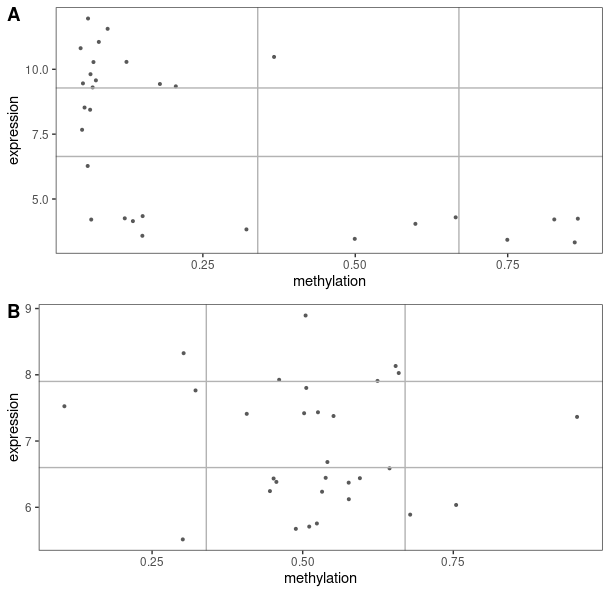
\includegraphics[width=0.5\textwidth,height=0.5\textheight]{figures/Figure1.png}
\caption{Example of non-Lshape vs L-shape for the
methylation--expression scatterplots associated with two real genes. A
represents a gene potentially regulated by methylation as expression
decreases with increasing methylation, giving a L--shaped scatterplot
that can be graphycally selected. B represents a gene not regulated by
methylation, since no correlation between expression and methylation
values is visible.}\label{id}
}
\end{figure}

\begin{figure}
\hypertarget{id}{%
\centering
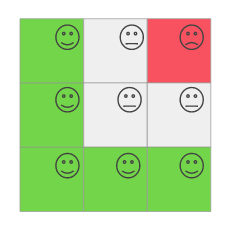
\includegraphics[width=0.5\textwidth,height=0.3\textheight]{figures/Figure2.png}
\caption{Grid representation to select L--shaped genes. A grid was
superimposed on the methylation--expression scatterplot graphs, each
cell representing one ninth of the graph. The grid partitioning of the
scatterplot was used to weigh the sample points so that sample points on
green cells would score higher whereas sample points on the red cell
would be penalized. Sample points distributed on the grey cells would be
given intermediatte weights.}\label{id}
}
\end{figure}

\begin{figure}
\hypertarget{id}{%
\centering
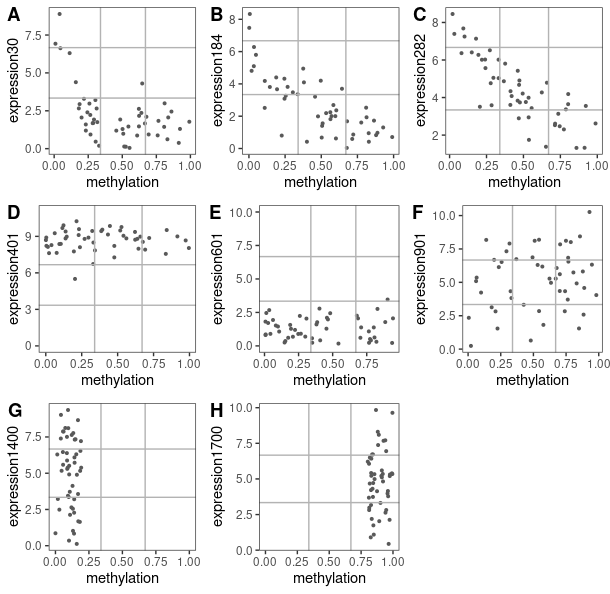
\includegraphics[width=0.9\textwidth,height=0.5\textheight]{figures/Figure3.png}
\caption{Representation of the 3 L--shaped vs the 5 non-L--shape
methylation--expression scatterplots from the artificially generated
genes. Figures A--C represent L--shaped genes and figures D--H represent
various patterns form non--L shaped genes. Subtle differences in
L--shaped genes are to assign correct weigth to the grid for the right
grouping toward L or non--L. Gene represented in A has the 4 top right
cells empty, gene in B has a similar oint distribution in the center
cell and in the bottom left cell, and gene in C has the bottom left cell
empty, and follows a stronger negative linear pattern. For the non--L
patterns, there is the D top distribution, E bottom distribution, F no
pattern, G left distribution, and H right distribution.}\label{id}
}
\end{figure}

\begin{figure}
\hypertarget{id}{%
\centering
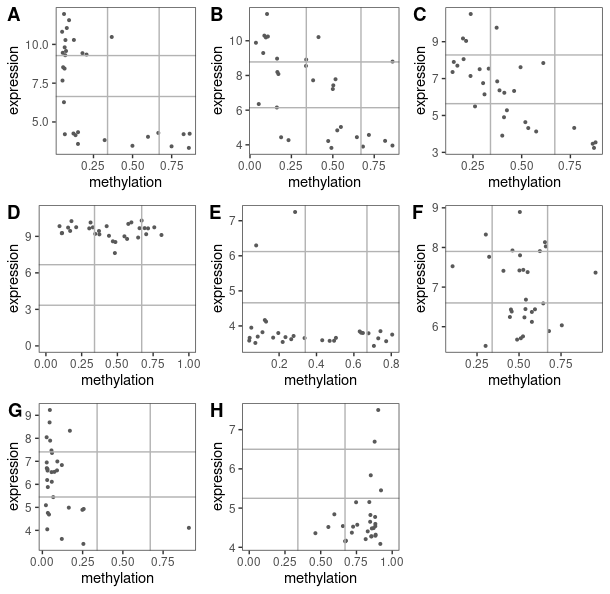
\includegraphics[width=0.9\textwidth,height=0.5\textheight]{figures/Figure4.png}
\caption{Representation of the 3 L--shaped vs the 5 non-L--shaped
methylation--expression scatterplots from real genes. Figures A--C
represent L--shaped genes and figures D--H represent various patterns
form non--L shaped genes. Following the same order of representation as
above.}\label{id}
}
\end{figure}

\begin{figure}
\hypertarget{id}{%
\centering
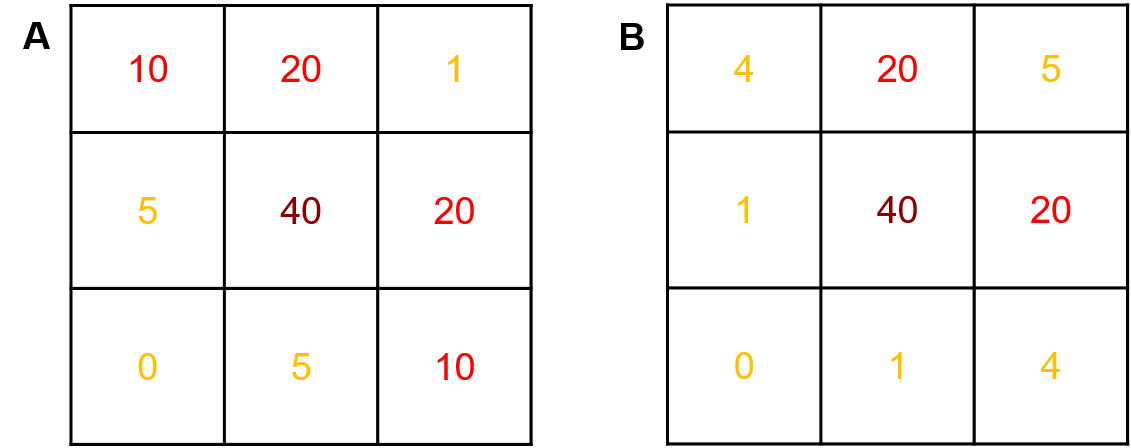
\includegraphics[width=0.7\textwidth,height=0.2\textheight]{figures/Figure5.png}
\caption{Percentage matrix used for datasets with different sample
sizes: (A) TCGA dataset, (B) Experimental dataset.}\label{id}
}
\end{figure}

\hypertarget{refs}{}
\begin{CSLReferences}{0}{0}
\leavevmode\hypertarget{ref-Berger2009}{}%
\CSLLeftMargin{1. }
\CSLRightInline{Berger SL, Kouzarides T, Shiekhattar R, Shilatifard A.
{An operational definition of epigenetics}. Genes and Development.
2009;23: 781--783.
doi:\href{https://doi.org/10.1101/gad.1787609}{10.1101/gad.1787609}}

\leavevmode\hypertarget{ref-Saxonov2006}{}%
\CSLLeftMargin{2. }
\CSLRightInline{Saxonov S, Berg P, Brutlag DL. {A genome-wide analysis
of CpG dinucleotides in the human genome distinguishes two distinct
classes of promoters}. Proceedings of the National Academy of Sciences
of the United States of America. 2006;103: 1412--1417.
doi:\href{https://doi.org/10.1073/pnas.0510310103}{10.1073/pnas.0510310103}}

\leavevmode\hypertarget{ref-Reik2007}{}%
\CSLLeftMargin{3. }
\CSLRightInline{Reik W. {Stability and flexibility of epigenetic gene
regulation in mammalian development}. Nature Publishing Group; 2007. pp.
425--432.
doi:\href{https://doi.org/10.1038/nature05918}{10.1038/nature05918}}

\leavevmode\hypertarget{ref-Portela2010}{}%
\CSLLeftMargin{4. }
\CSLRightInline{Portela A, Esteller M. {Epigenetic modifications and
human disease}. 2010. pp. 1057--1068.
doi:\href{https://doi.org/10.1038/nbt.1685}{10.1038/nbt.1685}}

\leavevmode\hypertarget{ref-Feil2012}{}%
\CSLLeftMargin{5. }
\CSLRightInline{Feil R, Fraga MF. {Epigenetics and the environment:
Emerging patterns and implications}. 2012. pp. 97--109.
doi:\href{https://doi.org/10.1038/nrg3142}{10.1038/nrg3142}}

\leavevmode\hypertarget{ref-Benayoun2015}{}%
\CSLLeftMargin{6. }
\CSLRightInline{Benayoun BA, Pollina EA, Brunet A. {Epigenetic
regulation of ageing: Linking environmental inputs to genomic
stability}. Nature Publishing Group; 2015. pp. 593--610.
doi:\href{https://doi.org/10.1038/nrm4048}{10.1038/nrm4048}}

\leavevmode\hypertarget{ref-Jones2002}{}%
\CSLLeftMargin{7. }
\CSLRightInline{Jones PA, Baylin SB. {The fundamental role of epigenetic
events in cancer}. 2002. pp. 415--428.
doi:\href{https://doi.org/10.1038/nrg816}{10.1038/nrg816}}

\leavevmode\hypertarget{ref-Feinberg1983}{}%
\CSLLeftMargin{8. }
\CSLRightInline{Feinberg AP, Vogelstein B. {Hypomethylation
distinguishes genes of some human cancers from their normal
counterparts}. Nature. 1983;301: 89--92.
doi:\href{https://doi.org/10.1038/301089a0}{10.1038/301089a0}}

\leavevmode\hypertarget{ref-Yang2014}{}%
\CSLLeftMargin{9. }
\CSLRightInline{Yang X, Han H, DeCarvalho DD, Lay FD, Jones PA, Liang G.
{Gene body methylation can alter gene expression and is a therapeutic
target in cancer}. Cancer Cell. Cell Press; 2014;26: 577--590.
doi:\href{https://doi.org/10.1016/j.ccr.2014.07.028}{10.1016/j.ccr.2014.07.028}}

\leavevmode\hypertarget{ref-McInnes2017}{}%
\CSLLeftMargin{10. }
\CSLRightInline{McInnes Tyler, Zou Donghui, Rao Dasari S., Munro
Francesca M., Phillips Vicky L., McCall John L., et al. {Genome-wide
methylation analysis identifies a core set of hypermethylated genes in
CIMP-H colorectal cancer}. BMC Cancer. 2017;17: 228.
doi:\href{https://doi.org/10.1186/s12885-017-3226-4}{10.1186/s12885-017-3226-4}}

\leavevmode\hypertarget{ref-Dong2019}{}%
\CSLLeftMargin{11. }
\CSLRightInline{Dong Lixin, Ma Li, Ma Gloria H., Ren H. {Genome-wide
Analysis Reveals DNA Methylation Alterations in Obesity Associated with
High Risk of Colorectal Cancer}. Scientific Reports. 2019;9: 5100.
doi:\href{https://doi.org/10.1038/s41598-019-41616-0}{10.1038/s41598-019-41616-0}}

\leavevmode\hypertarget{ref-Orjuela2020}{}%
\CSLLeftMargin{12. }
\CSLRightInline{Orjuela Stephany, Menigatti Mirco, Schraml Peter,
Kambakamba Patryk, Robinson Mark D., Marra G. {The DNA hypermethylation
phenotype of colorectal cancer liver metastases resembles that of the
primary colorectal cancers}. BMC Cancer. 2020;20: 290.
doi:\href{https://doi.org/10.1186/s12885-020-06777-6}{10.1186/s12885-020-06777-6}}

\leavevmode\hypertarget{ref-Zhang2010}{}%
\CSLLeftMargin{13. }
\CSLRightInline{Zhang Y, Jeltsch A. {The application of next generation
sequencing in DNA methylation analysis}. 2010. pp. 85--101.
doi:\href{https://doi.org/10.3390/genes1010085}{10.3390/genes1010085}}

\leavevmode\hypertarget{ref-Wreczycka2017}{}%
\CSLLeftMargin{14. }
\CSLRightInline{Wreczycka K, Gosdschan A, Yusuf D, Grüning B, Assenov Y,
Akalin A. {Strategies for analyzing bisulfite sequencing data}. Journal
of Biotechnology. 2017;261: 105--115.
doi:\href{https://doi.org/10.1016/j.jbiotec.2017.08.007}{10.1016/j.jbiotec.2017.08.007}}

\leavevmode\hypertarget{ref-Sadikovic2008}{}%
\CSLLeftMargin{15. }
\CSLRightInline{Sadikovic B, Al-Romaih K, Squire J A, Zielenska M. Cause
and consequences of genetic and epigenetic alterations in human cancer.
Current Genomics. 2008;9: 394--408.
doi:\href{https://doi.org/10.2174/138920208785699580}{10.2174/138920208785699580}}

\leavevmode\hypertarget{ref-Anastasiadi2018}{}%
\CSLLeftMargin{16. }
\CSLRightInline{Anastasiadi D, Esteve-Codina A, Piferrer F. {Consistent
inverse correlation between DNA methylation of the first intron and gene
expression across tissues and species}. Epigenetics and Chromatin.
BioMed Central Ltd.; 2018;11.
doi:\href{https://doi.org/10.1186/s13072-018-0205-1}{10.1186/s13072-018-0205-1}}

\leavevmode\hypertarget{ref-Massie2017}{}%
\CSLLeftMargin{17. }
\CSLRightInline{Massie CE, Mills IG, Lynch AG. The importance of DNA
methylation in prostate cancer development. The Journal of Steroid
Biochemistry and Molecular Biology. 2017;166: 1--15.
doi:\url{https://doi.org/10.1016/j.jsbmb.2016.04.009}}

\leavevmode\hypertarget{ref-Long2017}{}%
\CSLLeftMargin{18. }
\CSLRightInline{Long MD, Smiraglia DJ, Campbell MJ. {The Genomic Impact
of DNA CpG Methylation on Gene Expression; Relationships in Prostate
Cancer.} Biomolecules. Multidisciplinary Digital Publishing Institute
(MDPI); 2017;7.
doi:\href{https://doi.org/10.3390/biom7010015}{10.3390/biom7010015}}

\leavevmode\hypertarget{ref-Klett2018}{}%
\CSLLeftMargin{19. }
\CSLRightInline{Klett Hagen, Balavarca Yesilda, Toth Reka, Gigic
Biljana, Habermann Nina, Scherer Dominique, et al. Robust prediction of
gene regulation in colorectal cancer tissues from DNA methylation
profiles. Epigenetics. 2018;13: 386--397.
doi:\href{https://doi.org/10.1080/15592294.2018.1460034}{10.1080/15592294.2018.1460034}}

\leavevmode\hypertarget{ref-Sanchez-Pla2017}{}%
\CSLLeftMargin{20. }
\CSLRightInline{Sánchez-Pla Alex, Ruíz de Villa M. Carme, Carmona
Francesc, Bazzoco Sarah, del Corro DA. Integrative analysis to select
genes regulated by methylation in a cancer colon study. Ainsbury
Elizabeth A., Calle M.Luz, Cardis Elisabeth, Einbeck Jochen, Gómez
Guadalupe, Puig P, editors. Springer International Publishing; 2017. pp.
53--57. doi:\url{https://doi.org/10.1007/978-3-319-55639-0_9}}

\leavevmode\hypertarget{ref-Liu2012}{}%
\CSLLeftMargin{21. }
\CSLRightInline{Liu Y, Qiu P. Integrative analysis of methylation and
gene expression data in TCGA. Proceedings 2012 IEEE international
workshop on genomic signal processing and statistics (GENSIPS). 2012.
pp. 1--4.
doi:\href{https://doi.org/10.1109/GENSIPS.2012.6507712}{10.1109/GENSIPS.2012.6507712}}

\leavevmode\hypertarget{ref-Barat2015}{}%
\CSLLeftMargin{22. }
\CSLRightInline{Barat A, Ruskin H, Byrne A, Prehn J. {Integrating Colon
Cancer Microarray Data: Associating Locus-Specific Methylation Groups to
Gene Expression-Based Classifications}. Microarrays. MDPI AG; 2015;4:
630--646.
doi:\href{https://doi.org/10.3390/microarrays4040630}{10.3390/microarrays4040630}}

\leavevmode\hypertarget{ref-Koch2019}{}%
\CSLLeftMargin{23. }
\CSLRightInline{Koch A, Jeschke J, Van Criekinge W, Engeland M van, De
Meyer T. {MEXPRESS update 2019}. Nucleic Acids Research. 2019;47:
W561--W565.
doi:\href{https://doi.org/10.1093/nar/gkz445}{10.1093/nar/gkz445}}

\leavevmode\hypertarget{ref-Cedoz2018}{}%
\CSLLeftMargin{24. }
\CSLRightInline{Cedoz Pierre-Louis, Prunello Marcos, Brennan Kevin,
Gevaert O. MethylMix 2.0: An r package for identifying DNA methylation
genes. Bioinformatics. 2018;34: 3044--3046.
doi:\href{https://doi.org/10.1093/bioinformatics/bty156}{10.1093/bioinformatics/bty156}}

\leavevmode\hypertarget{ref-Silva2018}{}%
\CSLLeftMargin{25. }
\CSLRightInline{Silva TC GN Coetzee SG. ELMER v.2: An r/bioconductor
package to reconstruct gene regulatory networks from DNA methylation and
transcriptome profiles. Bioinformatics. 2018;35: 1974-\/-1977.
doi:\href{https://doi.org/10.1093/bioinformatics/bty902}{10.1093/bioinformatics/bty902}}

\leavevmode\hypertarget{ref-Huang2021}{}%
\CSLLeftMargin{26. }
\CSLRightInline{Huang H-Y, Li J, Tang Y, Huang Y-X, Chen Y-G, Xie Y-Y,
et al. {MethHC 2.0: information repository of DNA methylation and gene
expression in human cancer}. Nucleic Acids Research. 2020;49:
D1268--D1275.
doi:\href{https://doi.org/10.1093/nar/gkaa1104}{10.1093/nar/gkaa1104}}

\leavevmode\hypertarget{ref-Ongenaert2007}{}%
\CSLLeftMargin{27. }
\CSLRightInline{Ongenaert M, Van Neste L, De Meyer T, Menschaert G,
Bekaert S, Van Criekinge W. {PubMeth: a cancer methylation database
combining text-mining and expert annotation}. Nucleic Acids Research.
2007;36: D842--D846.
doi:\href{https://doi.org/10.1093/nar/gkm788}{10.1093/nar/gkm788}}

\end{CSLReferences}

\nolinenumbers


\end{document}
